\documentclass{beamer}
%
% Choose how your presentation looks.
%
% For more themes, color themes and font themes, see:
% http://deic.uab.es/~iblanes/beamer_gallery/index_by_theme.html
%

\usepackage{graphics}  % seems to be unnecessary in beamer
\usepackage{color,tikz}  % color seems to be unnecessary in beamer
\usepackage{hyperref} % seems to be unnecessary in beamer
\usepackage{braket}
\usepackage[italicdiff]{physics}
%\usepackage{mandi} % contains a lot of math and physics stuff
%clash for package xcolor

\usepackage{pgfpages}
\setbeamertemplate{note page}[plain]
\setbeameroption{show notes on second screen=right}

\usepackage[sort&compress,numbers]{natbib}
\usepackage{bibentry}
\bibliographystyle{apalike}
\renewcommand{\footnotesize}{\tiny}
\mode<presentation>
{
  \usetheme{default}      % or try Darmstadt, Madrid, Warsaw, ...
  \usecolortheme{default} % or try albatross, beaver, crane, ...
  \usefonttheme{default}  % or try serif, structurebold, ...
  \setbeamertemplate{navigation symbols}{}
  \setbeamertemplate{caption}[numbered]
  \addtobeamertemplate{navigation symbols}{}{%
    \usebeamerfont{footline}%
    \usebeamercolor[fg]{footline}%
    \hspace{1em}%
    \insertframenumber/\inserttotalframenumber
}
} 

\usepackage[english]{babel}
\usepackage[utf8x]{inputenc}

\title[main_aps_template]{APS  Presentation template}
\author{Tejas A Shetty}
\institute{IIT Bombay}
\date{\today}
\AtBeginSubsection[]
{
  \begin{frame}<beamer>{Outline}
    \tableofcontents[currentsection,currentsubsection]
  \end{frame}
}
\begin{document}
\nobibliography{mylit}

\begin{frame}
  \titlepage
\begin{center}
  
\includegraphics[scale=0.2]{IITB_logo.png}  \\
  \tikz{\draw (0,0)--(10,0)}
\end{center}
\end{frame}



% Uncomment these lines for an automatically generated outline.
\begin{frame}{Outline}
  \tableofcontents
\end{frame}

\section{Introduction}

\begin{frame}{Introduction}

\begin{itemize}
  \item Your introduction goes here!
  \item Use \texttt{itemize} to organize your main points.
\end{itemize}

\vskip 1cm

\begin{block}{Examples}
Some examples of commonly used commands and features are included, to help you get started.\footnote{\bibentry{nielsen2004quantum}}
\end{block}

\end{frame}
\begin{frame}


\begin{itemize}
  \item<1-> Eggs
  \item<2-> Plants
    \note[item]<2>{Tell joke about plants.}
    \note[item]<2>{Make it short.}
  \item<3-> Animals
\end{itemize}

\end{frame}
\begin{frame}{test}
hello
\note{say "hello" now}
\end{frame}
\section{Some \LaTeX{} Examples}

\subsection{Tables and Figures}

\begin{frame}{Tables and Figures}

\begin{itemize}
\item Use \texttt{tabular} for basic tables --- see Table~\ref{tab:widgets}, for example.
\item You can upload a figure (JPEG, PNG or PDF) using the files menu. 
\item To include it in your document, use the \texttt{includegraphics} command (see the comment below in the source code).
\end{itemize}

% Commands to include a figure:
%\begin{figure}
%\includegraphics[width=\textwidth]{your-figure's-file-name}
%\caption{\label{fig:your-figure}Caption goes here.}
%\end{figure}

\begin{table}
\centering
\begin{tabular}{l|r}
Item & Quantity \\\hline
Widgets & 42 \\
Gadgets & 13
\end{tabular}
\caption{\label{tab:widgets}An example table.}
\end{table}

\end{frame}

\subsection{Mathematics}

\begin{frame}{Readable Mathematics}

Let $X_1, X_2, \ldots, X_n$ be a sequence of independent and identically distributed random variables with $\text{E}[X_i] = \mu$ and $\text{Var}[X_i] = \sigma^2 < \infty$, and let
$$S_n = \frac{X_1 + X_2 + \cdots + X_n}{n}
      = \frac{1}{n}\sum_{i}^{n} X_i$$
denote their mean. Then as $n$ approaches infinity, the random variables $\sqrt{n}(S_n - \mu)$ converge in distribution to a normal $\mathcal{N}(0, \sigma^2)$.

\end{frame}

% =================================================== 

\begin{frame}[t]
\vspace*{1cm}
 
Note: the content presented is just for the \textcolor{red}{\bf test}. \\
\texttt{Please bear with the simplicity :).}\\[0.4cm]
\begin{block}
{{\em Pythagoras Theorem} a special case of {\em Cauchy-Schwarz inequality} stated as (\ref{eqn1}).}
\end{block}

\begin{equation}
 |(\alpha+\beta)| \leq \sqrt{|\alpha|^2 + |\beta|^2} \label{eqn1}
\end{equation}
\vskip 1cm
where, $\alpha$, $\beta$ are two vectors in $\Re^n$.\\

\end{frame}

% ======================================================
 \begin{frame}[t]
\vspace{0.5cm}

\noindent Consider the trajectory\footnotemark[2] $$y = \sin(x) + 0.3\sin(3x)$$ over the range of [-$\pi$, $\pi$] is tabulated as shown:
\vskip 0.2cm

\begin{table}[h]
\begin{center} 
{
\begin{tabular}{cc}
\hline
$x$ (rad)	& $y$  		\\ \hline\hline
-$\pi$  	& -0.0000 	\\
-$3\pi/4$ 	& -0.9192	\\
-$2\pi/4$ 	& -0.7000 	\\ \hline
-$\pi/4$ 	& -0.9192	\\
0.0000  	& 0.0000 	\\
$\pi/4$  	& 0.9192	\\ \hline
$2\pi/4$ 	& 0.7000	\\
$3\pi/4$ 	& 0.9192	\\
$\pi$ 		& 0.0000 	\\\hline\hline
\end{tabular}}
\end{center}
\end{table}

\footnotetext[2]{trajectory can be a response.}
\end{frame}
% ========================================================
\begin{frame}
 
The plot for above table is as shown:\footnotemark[3]

\begin{minipage}[c]{1\textwidth}
\begin{center}
\resizebox{0.8\textwidth}{!}{
  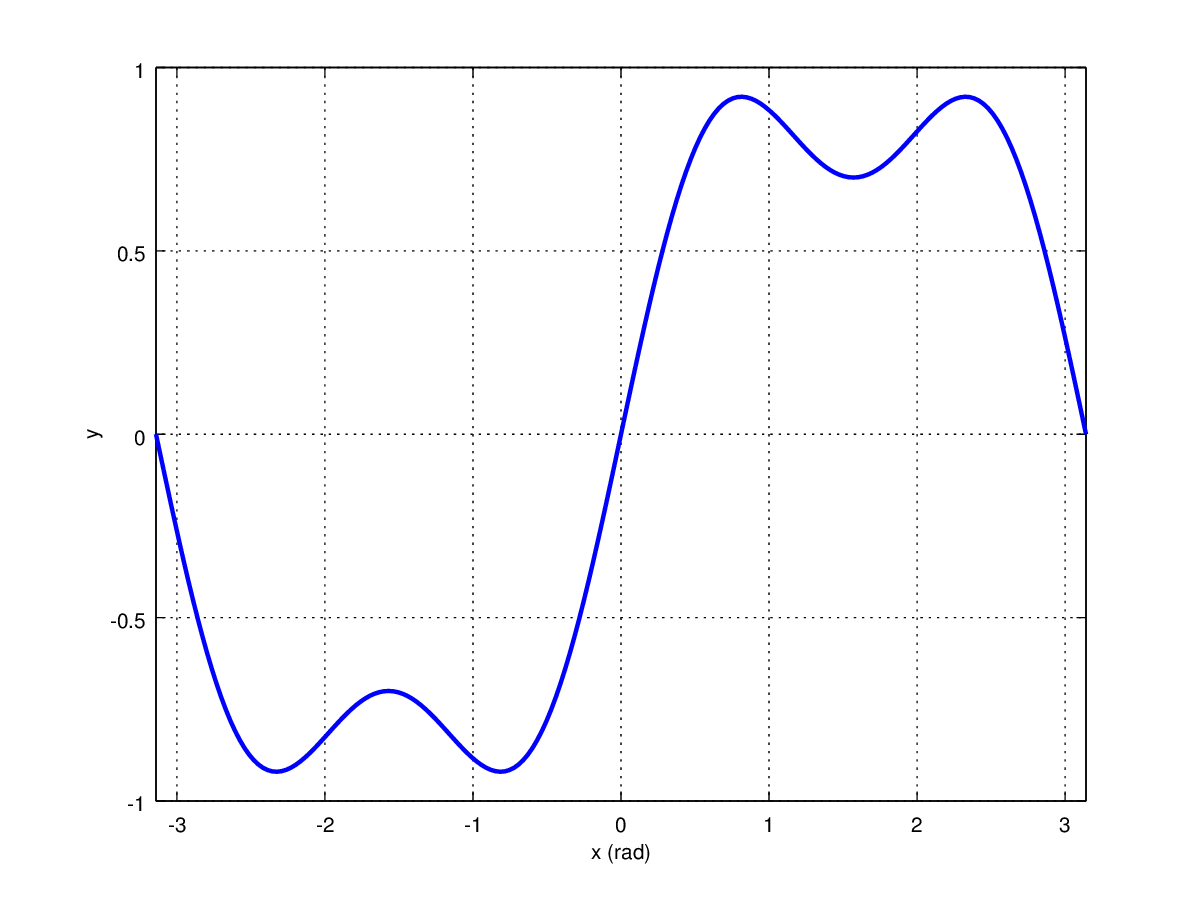
\includegraphics{traj_plot.png}  
}
\end{center}
\end{minipage}

Packages for PPT tested ... 
\footnotetext[3]{Use for citing references}
\end{frame}
% ========================================================

% ========================================================
\begin{frame}
 \Huge 
 \centering 
  That's all Folks!\\
  {\large See you in Workshop...}
\end{frame}


\end{document}
